\newcommand{\specname}{PanoSpec}
\newcommand{\status}{Beta}
\newcommand{\ecn}{NA}
\newcommand{\revdate}{120128}
\newcommand{\rev}{000}

\documentclass[dvips,12pt]{article}
\renewcommand{\contentsname}{3. Index} 

\usepackage{amsmath}
%\usepackage{program}
\usepackage{a4,color,graphics,palatino,fancyhdr}
\usepackage{lastpage}
\usepackage{fancyhdr}
\usepackage{changepage}% http://ctan.org/pkg/changepage
\usepackage{graphicx}

\setlength{\headheight}{15pt}

\setcounter{secnumdepth}{1}
\setcounter{tocdepth}{1}

\lhead{\specname}
\rhead{rev.\  \rev} 
\chead{\revdate}
\cfoot{\footnotesize Page\ \thepage\ of \pageref{LastPage}}
\pagestyle{fancy}
\title{PanoSpec}

\author{chaz}

\begin{document}

\frenchspacing

%\renewcommand{\arraystretch}{1.4}% adjust hline heights for prettiness
%\begin{adjustwidth}{-.03in}{-.1in}% adjust the L and R margins by 1 inch
%\begin{tabular}{|l|l|}
%\hline
%pic & nothing & stuff\\
%\hline
%Spec Name:\ \specname & Revision:\ \rev \\
%\hline
%Spec Status:\ \status & Effective Date:\ \revdate \\
%\hline
%\end{tabular}
%\end{adjustwidth}

\section{Purpose}
Documentation for panoramicam

\tableofcontents
\listoffigures

\renewcommand{\arraystretch}{1}
\section{References}
\begin{adjustwidth}{2.5em}{0pt}
\begin{tabular}{ l  l }
panoramicalcs.ods & Documention spreadsheet \\
Allegro A4988  & datasheet\\
\end{tabular}
\end{adjustwidth}

\section{Definitions}
\begin{adjustwidth}{2.5em}{0pt}
\begin{description}
    \item[theta] The angle of the platform, referenced to the start position
    \item[phi] The angle of the film spool, referenced from the start position
    \item[base] The stationary part of panoramicam, which attaches to the tripod
    \item[platform]The rotationary part of panoramicam, which holds the camera
\end{description}
\end{adjustwidth}

\section{Panoramicam}

\subsection{The slit-scan camera concept}
A slit-scan camera is a type of panoramic camera that makes a continuous exposure while panning horizontally. As the image moves across the focal plane, the film is moved through the gate at the same speed as the image. The result is a panoramic image of 360 degrees or more with a unique perspective. To reduce smearing from perspective distortion and to reduce exposure, a mask is typically placed in the film gate, blocking the image but for a thin vertical slot.

\begin{figure}
\centering
includegraphics[width=0.8\textwidth]{test}
\caption{Panoramicam}
\label{fig:Panoramicam}
\end{figure}

The concept of a scanning-type camera is not new. The Cirkut camera was scanning camera that was produced around 1905. It used large-format roll film and mechanical clockwork to take panoramic images of up to 360 degrees. The large negatives were then contact printed in the darkroom. These cameras are now rare and expensive, and if film is still available, it will not be for long. Scanning-type cameras have also been used to deliberately create distorted images for motion picture special effects, such as the ``warp effect'' from \emph{Star Trek} and the ending bit of \emph{2001: A Space Odyssey.}

\subsection{Implementation details}

The goal of the Panoramicam project was to create a slit-scanning camera for my own use, which fits into my photographic workflow, and which uses currently-available film.

In designing Panoramicam, I first considered using 120 film, which is essentially a miniature version of the large-format film used by the Cirkut camera, and still widely available. However, 120 film generates contact prints which are quite small and unimpressive, and enlarging a panoramic negative would be impossible without either a 10x10 enlarger or building a special slit-scanning projection printer. 

The enlarging requirement led to the use of 35mm film. With 35mm film, a wide-ratio negative can be enlarged using a common 4x5 enlarger. The use of such small film imposes some technical limitations, but those limitations are somewhat mitigated by the fact that the camera design allows generous exposure, so that fine-grained film can be used at all times. 

If digital output is acceptable, the film can easily be scanned using currently existing technology. Of course, this would also be the case for 120-size film, but I am specifically interested in chemical photography, and I prefer to work with silver, having only academic interest in digital imaging. Where a digital image is acceptable, a common panoramic technique is to stitch multiple files from a digital camera into a panorama; something which is widely done. But the continuous nature of the scanning camera's exposure provides images with a dynamic nature different from images generated from multiple still images.


\begin{figure}[htb]
    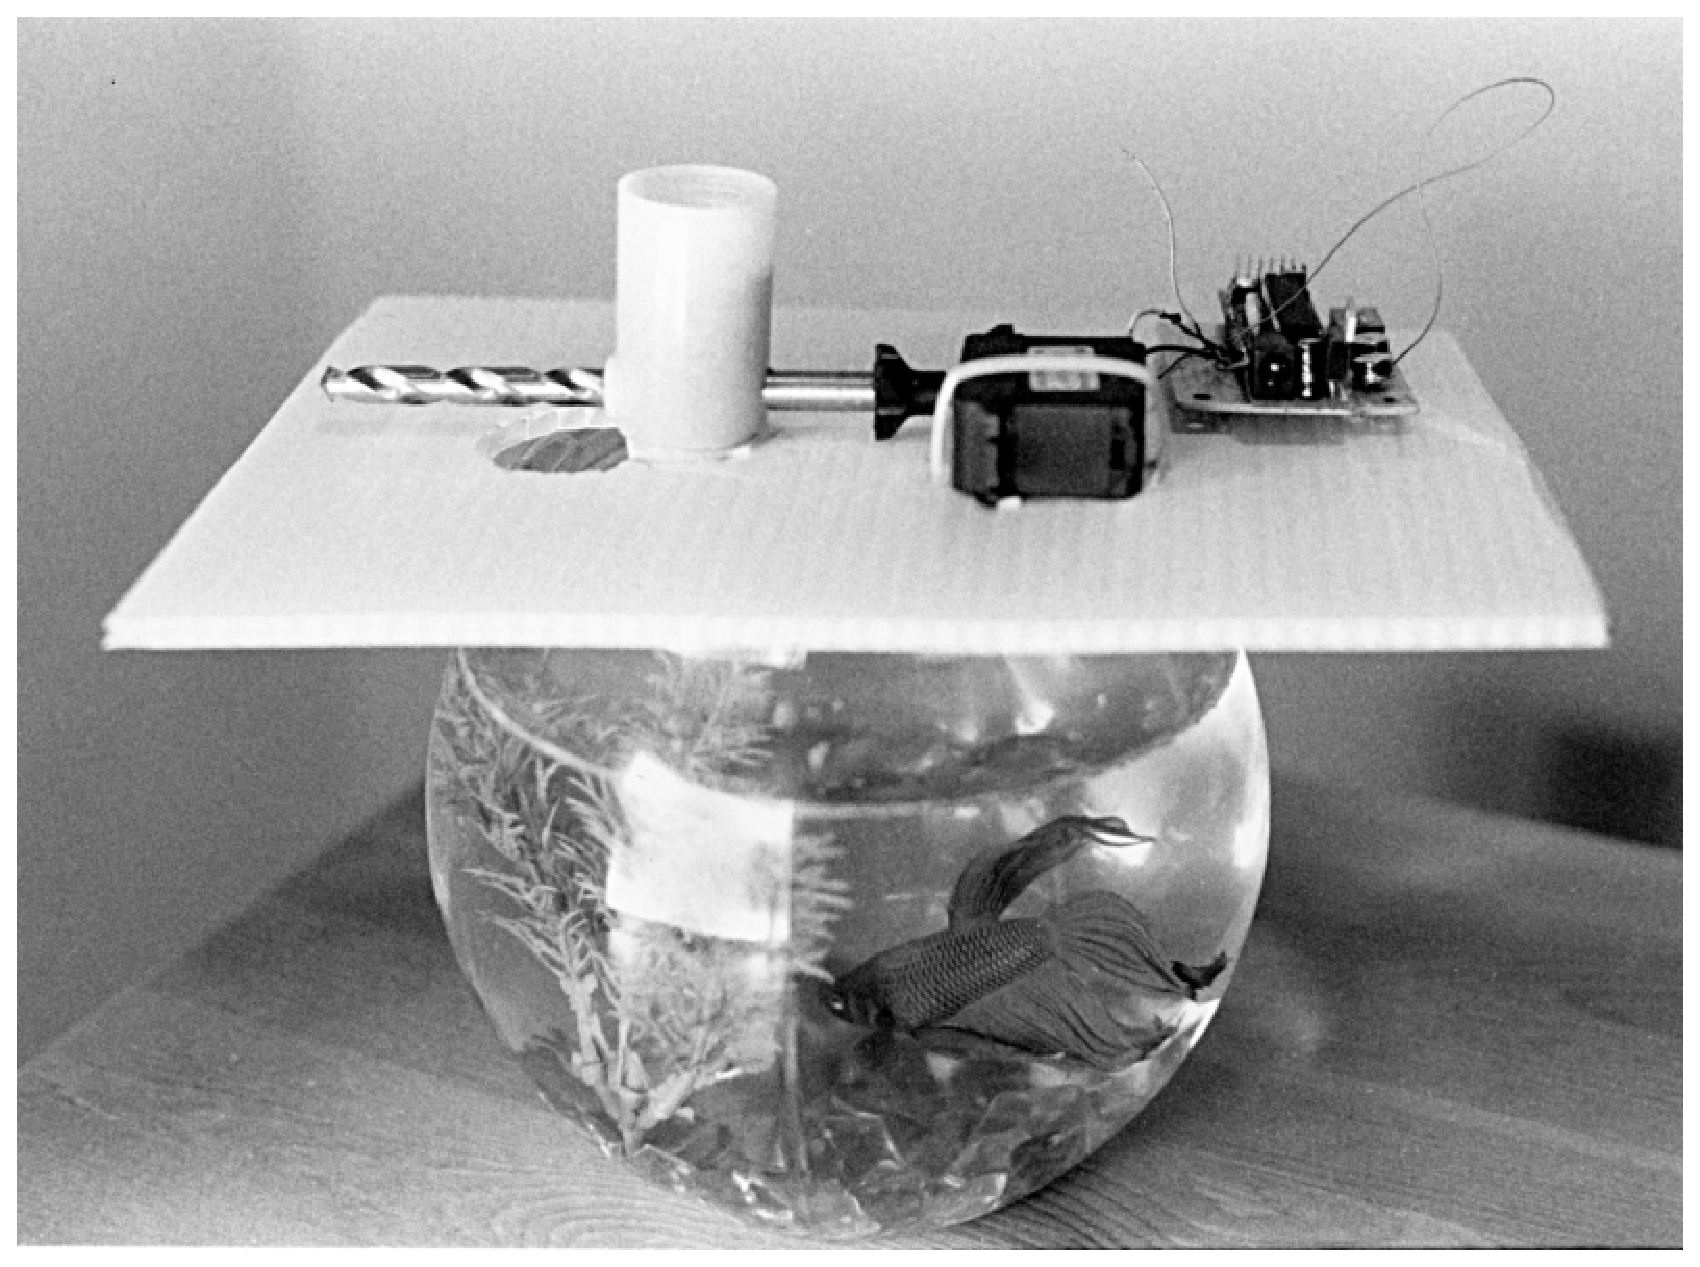
\includegraphics[width=0.8\textwidth]{test}
    \caption{Panoramicam II}
    \label{fig:pano}
\end{figure}

\begin{figure}[htb]
\centering
\setlength{\unitlength}{1cm}

    \begin{picture}(12,8)
	\centering
	\thicklines

	\put(0,0){\line(1,0){12}}
	\put(0,0){\line(0,1){8}}
	\put(12,0){\line(0,1){8}}
	\put(0,8){\line(1,0){12}}
	\put(2,2){\line(1,0){8}}
	\put(5.7,2.2){\line(1,6){.7}}

	\put(2, 2){\vector(1, 0){8}}
	\put(6, 2){\vector(0,1){5.5}}
	\put(4.5,4.22){\vector(1,0){.75}}
	%\put(5.5,1.7){\vector(1,0){.5}}
	\put(5.6,1.74){$\leftrightarrow$}

	\put(6.5,5.7){\math d\theta\)}
	\put(5.55,1.4){\math dx\)}
	%dx=f \cdot d\theta$}

	\put(10,2.2){$x$}
	\put(6.2,7.4){$y$}
	\put(1,6.5){\large $Top\ View$}
	\put(2.7,4.1){\footnotesize $Exit\ Pupil$}
	\put(2,2.1){\footnotesize $Film Plane$}

	\qbezier(6,5.8)(6.2,6)(6.3,5.75)
	\put(6, 4.2){\circle{.666666}}

    \end{picture}
    \caption{Theta}
    \label{fig:theta}
\end{figure}


\begin{figure}[htb]
    \centering
    \setlength{\unitlength}{1cm}
\begin{picture}(12,8)
    \centering
    \thicklines

    \put(0,0){\line(1,0){12}}
    \put(0,8){\line(1,0){12}}
    \put(0,0){\line(0,1){8}}
    \put(12,0){\line(0,1){8}}

    \thicklines
    \put(4,2){\vector(1,0){6}}

    \put(4, 4){\circle{9}}
    %\put(4.1, 3.9){$\leftrightarrow$}
    \put(4, 4){\vector(1, 0){.65}}
    \put(4, 4){\vector(0,-1){2}}

    
    %circle at x=4, y=4, with diameter 4
    %8 bezier primitives used
    \qbezier (6.000,4.000)(6.000,4.828)(5.414,5.414)
    \qbezier (5.414,5.414)(4.828,6.000)(4.000,6.000)
    \qbezier (4.000,6.000)(3.172,6.000)(2.586,5.414)
    \qbezier (2.586,5.414)(2.000,4.828)(2.000,4.000)
    \qbezier (2.000,4.000)(2.000,3.172)(2.586,2.586)
    \qbezier (2.586,2.586)(3.172,2.000)(4.000,2.000)
    \qbezier (4.000,2.000)(4.828,2.000)(5.414,2.586)
    \qbezier (5.414,2.586)(6.000,3.172)(6.000,4.000)

    \put(4.2,4.1){\math r\)}
    \put(4.1,2.6){\math R\)}
    \put(10,2.2){\math x\)}
    \put(3.6,4){\large \math \phi\)}
    \put(8, 1.5){\large \math film \)}

    \put(1,6.5){\large $Top\ View$}

\end{picture}

\caption{Phi}
\label{fig:phi}
\end{figure}

\renewcommand{\arraystretch}{1.4}% adjust hline heights for prettiness
\begin{figure}[htb]
\centering
\begin{tabular}{|c|c|c|c|c|c|}
\hline
S3&S2&S1&Rotation Period&T, 28mm lens, s&T, 50mm lens, s\\
\hline
0&0&0&8 seconds&1/16&1/30\\
\hline
0&0&1&16 seconds&1/8&1/15\\
\hline
0&1&0&32 seconds&1/4&1/8\\
\hline
0&1&1&64 seconds&1/2&1/4\\
\hline
1&0&0&10 minutes&6&3\\
\hline
1&0&1&20 minutes&12&6\\
\hline
1&1&0&1 hour&60&30\\
\hline
1&1&1&4 hours&120&60\\
\hline
\end{tabular}
\caption{Exposure-DIP switch table}
\label{fig:exposure}
\end{figure}
%
%\begin{figure}[htb]
%\centering
%\includegraphics[width=0.8\textwidth]{test2}
%\caption{Awesome Image 2}
%\label{fig:awesome_image}
%\end{figure}

\section{Theoretical Development}

The essential requirement of the slit-scan camera is this: the speed at which the film is moved through the film gate must equal the speed at which the image moves across the focal plane. If this synchronization is not maintained, the image will not be sharp. 
The speed of the image doesn't change during the exposure, because the camera rotates with a constant speed for an even exposure. However, we can see that if we pull the film by wrapping it around a spool, the effective diameter of the spool will change as the film winds on, and so the speed of the film-pulling will increase as the exposure proceeds. A capstan drive or a ``large'' takeup spool would mitigate this concern. Another option would be to directly sense film speed (somehow) and use servo feedback to maintain the film speed, but since I opted to build Panoramicam from an existing 35mm camera, my best option was to model the film-piling and continuously change the winding speed in an ``open-loop'' manner in order to keep synchronization lock between the image speed and film speed. This turns out to work quite well. 

Referring to figure~\ref{fig:theta}, and considering a small angle, we can see that the image speed, \math \dot{x} \), depends on the panning rate, \math \dot{\theta} \) and the focal length of the lens,\math f \), expressed thusly:

\begin{displaymath}
\dot{x} = f \cdot \dot{\theta }
\end{displaymath}

Referring to figure~\ref{fig:phi} we can see that the linear film speed, \math \dot{x}\) , depends on the turning rate of the takeup spool, \math \dot{\phi}\), and the instantaneous diameter of the takeup spool, \math R\), which itself is determined by the film thickness, \math t\), the starting spool diameter, \math r\), and the instantaneous total angle turned by the film spool, \math \phi \), expressed thusly:

\begin{displaymath}
\dot{x} = \dot{\phi} \left( r+\frac{t\theta}{2\pi}\right)
\end{displaymath}

Thus in operation, the speed of the film winding spool, \math \dot{\theta} \), must be maintained as

\begin{displaymath}
\dot{\phi} = \frac{f\dot{\theta}}{\left(r+\frac{\theta t}{2 \pi}\right)}
\end{displaymath}

This establishes the `sync function' needed to implement the programming. Since common microcontrollers lack hardware for performing floating-point math, several simplifications are used in the actual algorithm. 

\section{Hardware description}
\subsection{The Camera}
Panoramicam uses a 35mm camera body as the core. An Olympus OM1 was chosen because it has a mechanical shutter, which allows the shutter to be locked open without draining the camera batteries. Also, the rewind control is located on the front of the camera, which simplifies operation. The designer also has a supply of OM-mount lenses. 
\subsection{The Platform}
The camera body is placed on a rotating platform so that the lens nodal point is centered over the pivot point for the platform. A stepper motor is interfaced to the film rewind crank with a M4 screw and coupling made from a 7mm socket. The stepper is quickly removable to allow the film to be changed. 
\subsection{The Base}
The base is formed from aluminum plate. The bearing assembly is built from laminated plastic and the bearings are bronze oillite type. 
\subsection{The Motion Control hardware}
At the platform, the film is wound by a bipolar stepper motor. An Allegro microstepping driver board is used to control the stepper, and an AVR ATMEGA168 is used with a Boarduino project board for control. A daughter board provides DIP switches and pushbuttons for human interface.

At the base, a unipolar stepper motor is interfaced to the platform through a neoprene timing belt at a gear reduction ratio of 6:1, giving 1200 full steps per platform revolution. The stepper is driven by a simple 4-transistor driver board, which is in turn controlled by another AVR microcontroller. To provide smooth motion, the motor is driven as a high-pole-count AC synchronous motor by sine waves synthesized by the microcontroller's PWM output. A daughter board provides buttons and DIP switches for human interface.

\section{Operating Instructions}

\subsection{Initial Setup}
\begin{enumerate}
\item Ensuring the batteries are charged, power up both the platform and the base. Check the green LEDs and make sure the microcontrollers are powered up.
\item Choose platform rotation period and enter the DIP switch settings on the base daughter board. Consult table~\ref{fig:exposure} for help choosing exposure.
\item Enter the same settings on the platform daughter board. If these DIP switch settings don't match between the platform and the base, interesting psychedelic smearing will occur in the images.
\item Set switch 4 according to the lens installed. See the previous note on psychedelic smearing. 
\item Using the manual input buttons, rotate the platform to the orientation in which you would like to begin exposure. 
\end{enumerate}

\subsection{Load the film}
\begin{enumerate}
\item Determine if there is film in the camera already. There is no good way to determine this, so take notes. You could always try rewinding it to be safe.
\item Remove the film motor and unlatch the camera back by pulling up on the spool drive.
Load the film in the usual way.
\item Close the back, fit the lens cap and fire the entire roll using the motor drive.
\item Fit the film motor back on and ensure it fits on the spool drive. Using the motor drive buttons, turn the spool drive 1/2 turn to take up film slack.
\end{enumerate}

\subsection{Make The Exposure}
\begin{enumerate}
\item To begin exposure, press the start buttons on both the platform and the base at the same time (within 1 second).
\item To stop the exposure, or to abort, yank the power cords.
\end{enumerate}

\section{Software Functional Spec}

The relationships derived in the theoretical development section above serve to fundamentally describe the camera operation. In implementing the software, the sync function can't be implement directly in C due to hardware limitations of 8-bit microcontrollers, which have no floating-point unit and operate with limited clock speed and memory. In practice, all the linear variables are lumped to quantities which correspond directly to the timer registers of the microcontroller, and the sync function is approximated using its Taylor series expansion. 

\subsection{Basic Software Function}

\subsubsection{Base}
Drive the platform smoothly at a variety of speeds. Provide a user interface that allows different speeds to be chosen and allow the user to pre-position the platform.

\subsubsection{Platform}
Drive the film motor smoothly at precisely the right speed to capture sharp images. Vary the speed of the film spool to compensate for increased diameter as the film winds on. Keep track of the amount of film wound on, to allow multiple exposures on the same roll. Provide a human interface that allows different speeds to be chosen and the lens to be specified. Allow the user to manually control the motor for setup.

\subsection{Software Requirements}
\subsubsection{Inputs and Outputs}


\renewcommand{\arraystretch}{1.4}% adjust hline heights for prettiness
\begin{figure}[htb]
\centering
\begin{tabular}{|c|c|c|}
\hline
Input&Function&AVR PORT pin\\
\hline
Left&Rotate Left&D0\\
\hline
Start&Start Pictionation&D1\\
\hline
Right&Rotate Right&D2\\
\hline
DIP 0&Speed Select&C0\\
\hline
DIP 1&Speed Select&C1\\
\hline
DIP 2&Speed Select&C2\\
\hline
DIP 3&Speed Select&C3\\
\hline
DIP 4&Lens Selector&C4\\
\hline
\end{tabular}
\caption{Platform Inputs}
\label{fig:platforminputs}
\end{figure}

\renewcommand{\arraystretch}{1.4}% adjust hline heights for prettiness
\begin{figure}[htb]
\centering
\begin{tabular}{|c|c|c|}
\hline
Output&Function&AVR PORT pin\\
\hline
Step&Step Motor&B0\\
\hline
Dir&Set Motor Direction&B2\\
\hline
LED&Blinkenled&B5\\
\hline
\end{tabular}
\caption{Platform Outputs}
\label{fig:platformoutputs}
\end{figure}

\renewcommand{\arraystretch}{1.4}% adjust hline heights for prettiness
\begin{figure}[htb]
\centering
\begin{tabular}{|c|c|c|}
\hline
Input&Function&AVR PORT pin\\
\hline
Left&Rotate Left&D0\\
\hline
Right&Rotate Right&D1\\
\hline
Start&Start Pictionation&D2\\
\hline
DIP 0&Speed Select&C0\\
\hline
DIP 1&Speed Select&C1\\
\hline
DIP 2&Speed Select&C2\\
\hline
DIP 3&Speed Select&C3\\
\hline
\end{tabular}
\caption{Base Inputs}
\label{fig:baseinputs}
\end{figure}

\renewcommand{\arraystretch}{1.4}% adjust hline heights for prettiness
\begin{figure}[htb]
\centering
\begin{tabular}{|c|c|c|}
\hline
Output&Function&AVR PORT pin\\
\hline
Motor 1&Step Motor&OCR0A\\
\hline
Motor 2&Step Motor&OCR0B\\
\hline
Motor 3&Step Motor&OCR2A\\
\hline
Motor 4&Step Motor&OCR2B\\
\hline
LED&Blinkenled&B5\\
\hline
\end{tabular}
\caption{Base Outputs}
\label{fig:baseoutputs}
\end{figure}

\subsubsection{Human Interface}
The software will provide a user interface that allows either motor to be manually controlled for camera setup. The user will be able to select the operation speed through DIP switches. The user will be able to initiate pictionation sequence. 
\subsubsection{Motor Control}
The film motor will be controlled using step, dir interface described in the Allego datasheet (listed in references).

The platform motor will be driven directly using the 4-wire unipolar stepper motor interface from the driver board. A sine-wave drive will be implemented in software, using the PWM capability of the AVR ATMEGA168.
\subsubsection{Errors, Faults and Programmability}
Errors will be indicated with a blinkenled for diagnostics purposes.
\subsection{Development}
The programs will be written for the AVR ATMEGA microcontrollers using the GNU C compiler for the AVR (avr-gcc). The vi text editor will be used for development and git used for revision control. 


\section{Example Source code}
The source code shown here is for example only; it is provided as `pseudo-code` for the reader and is not necessarily up-to-date.
\subsection{platform example code}
\texttt{some code here}
\subsection{base example code}
\begin{verbatim}
ome    code % and st
uff
\end{verbatim}
\centering

\vspace{2cm}

END OF DATA
\appendix

\end{document}

